\documentclass[twoside]{book}

% Packages required by doxygen
\usepackage{calc}
\usepackage{doxygen}
\usepackage{graphicx}
\usepackage[utf8]{inputenc}
\usepackage{makeidx}
\usepackage{multicol}
\usepackage{multirow}
\usepackage{textcomp}
\usepackage[table]{xcolor}

% Font selection
\usepackage[T1]{fontenc}
\usepackage{mathptmx}
\usepackage[scaled=.90]{helvet}
\usepackage{courier}
\usepackage{amssymb}
\usepackage{sectsty}
\renewcommand{\familydefault}{\sfdefault}
\allsectionsfont{%
  \fontseries{bc}\selectfont%
  \color{darkgray}%
}
\renewcommand{\DoxyLabelFont}{%
  \fontseries{bc}\selectfont%
  \color{darkgray}%
}

% Page & text layout
\usepackage{geometry}
\geometry{%
  a4paper,%
  top=2.5cm,%
  bottom=2.5cm,%
  left=2.5cm,%
  right=2.5cm%
}
\tolerance=750
\hfuzz=15pt
\hbadness=750
\setlength{\emergencystretch}{15pt}
\setlength{\parindent}{0cm}
\setlength{\parskip}{0.2cm}
\makeatletter
\renewcommand{\paragraph}{%
  \@startsection{paragraph}{4}{0ex}{-1.0ex}{1.0ex}{%
    \normalfont\normalsize\bfseries\SS@parafont%
  }%
}
\renewcommand{\subparagraph}{%
  \@startsection{subparagraph}{5}{0ex}{-1.0ex}{1.0ex}{%
    \normalfont\normalsize\bfseries\SS@subparafont%
  }%
}
\makeatother

% Headers & footers
\usepackage{fancyhdr}
\pagestyle{fancyplain}
\fancyhead[LE]{\fancyplain{}{\bfseries\thepage}}
\fancyhead[CE]{\fancyplain{}{}}
\fancyhead[RE]{\fancyplain{}{\bfseries\leftmark}}
\fancyhead[LO]{\fancyplain{}{\bfseries\rightmark}}
\fancyhead[CO]{\fancyplain{}{}}
\fancyhead[RO]{\fancyplain{}{\bfseries\thepage}}
\fancyfoot[LE]{\fancyplain{}{}}
\fancyfoot[CE]{\fancyplain{}{}}
\fancyfoot[RE]{\fancyplain{}{\bfseries\scriptsize Generated on Thu Mar 10 2016 07\-:43\-:39 for My Project by Doxygen }}
\fancyfoot[LO]{\fancyplain{}{\bfseries\scriptsize Generated on Thu Mar 10 2016 07\-:43\-:39 for My Project by Doxygen }}
\fancyfoot[CO]{\fancyplain{}{}}
\fancyfoot[RO]{\fancyplain{}{}}
\renewcommand{\footrulewidth}{0.4pt}
\renewcommand{\chaptermark}[1]{%
  \markboth{#1}{}%
}
\renewcommand{\sectionmark}[1]{%
  \markright{\thesection\ #1}%
}

% Indices & bibliography
\usepackage{natbib}
\usepackage[titles]{tocloft}
\setcounter{tocdepth}{3}
\setcounter{secnumdepth}{5}
\makeindex

% Hyperlinks (required, but should be loaded last)
\usepackage{ifpdf}
\ifpdf
  \usepackage[pdftex,pagebackref=true]{hyperref}
\else
  \usepackage[ps2pdf,pagebackref=true]{hyperref}
\fi
\hypersetup{%
  colorlinks=true,%
  linkcolor=blue,%
  citecolor=blue,%
  unicode%
}

% Custom commands
\newcommand{\clearemptydoublepage}{%
  \newpage{\pagestyle{empty}\cleardoublepage}%
}


%===== C O N T E N T S =====

\begin{document}

% Titlepage & ToC
\hypersetup{pageanchor=false}
\pagenumbering{roman}
\begin{titlepage}
\vspace*{7cm}
\begin{center}%
{\Large My Project }\\
\vspace*{1cm}
{\large Generated by Doxygen 1.8.6}\\
\vspace*{0.5cm}
{\small Thu Mar 10 2016 07:43:39}\\
\end{center}
\end{titlepage}
\clearemptydoublepage
\tableofcontents
\clearemptydoublepage
\pagenumbering{arabic}
\hypersetup{pageanchor=true}

%--- Begin generated contents ---
\chapter{Hierarchical Index}
\section{Class Hierarchy}
This inheritance list is sorted roughly, but not completely, alphabetically\-:\begin{DoxyCompactList}
\item \contentsline{section}{Data\-\_\-set}{\pageref{classData__set}}{}
\item \contentsline{section}{data\-\_\-subset}{\pageref{structdata__subset}}{}
\item exception\begin{DoxyCompactList}
\item \contentsline{section}{invalid\-\_\-dataset\-\_\-exception}{\pageref{classinvalid__dataset__exception}}{}
\end{DoxyCompactList}
\item \contentsline{section}{Net\-\_\-benchmark}{\pageref{classNet__benchmark}}{}
\item \contentsline{section}{net\-\_\-topology}{\pageref{structnet__topology}}{}
\item \contentsline{section}{Neural\-Net}{\pageref{classNeuralNet}}{}
\item \contentsline{section}{Trainer}{\pageref{classTrainer}}{}
\begin{DoxyCompactList}
\item \contentsline{section}{Backpropagation\-\_\-trainer}{\pageref{classBackpropagation__trainer}}{}
\item \contentsline{section}{Evolutionary\-\_\-trainer}{\pageref{classEvolutionary__trainer}}{}
\end{DoxyCompactList}
\end{DoxyCompactList}

\chapter{Class Index}
\section{Class List}
Here are the classes, structs, unions and interfaces with brief descriptions\-:\begin{DoxyCompactList}
\item\contentsline{section}{\hyperlink{classBackpropagation__trainer}{Backpropagation\-\_\-trainer} }{\pageref{classBackpropagation__trainer}}{}
\item\contentsline{section}{\hyperlink{classData__set}{Data\-\_\-set} }{\pageref{classData__set}}{}
\item\contentsline{section}{\hyperlink{structdata__subset}{data\-\_\-subset} }{\pageref{structdata__subset}}{}
\item\contentsline{section}{\hyperlink{classEvolutionary__trainer}{Evolutionary\-\_\-trainer} }{\pageref{classEvolutionary__trainer}}{}
\item\contentsline{section}{\hyperlink{classinvalid__dataset__exception}{invalid\-\_\-dataset\-\_\-exception} }{\pageref{classinvalid__dataset__exception}}{}
\item\contentsline{section}{\hyperlink{classNet__benchmark}{Net\-\_\-benchmark} }{\pageref{classNet__benchmark}}{}
\item\contentsline{section}{\hyperlink{structnet__topology}{net\-\_\-topology} }{\pageref{structnet__topology}}{}
\item\contentsline{section}{\hyperlink{classNeuralNet}{Neural\-Net} \\*The \hyperlink{classNeuralNet}{Neural\-Net} class }{\pageref{classNeuralNet}}{}
\item\contentsline{section}{\hyperlink{classTrainer}{Trainer} }{\pageref{classTrainer}}{}
\end{DoxyCompactList}

\chapter{Class Documentation}
\hypertarget{classBackpropagation__trainer}{\section{Backpropagation\-\_\-trainer Class Reference}
\label{classBackpropagation__trainer}\index{Backpropagation\-\_\-trainer@{Backpropagation\-\_\-trainer}}
}


Inheritance diagram for Backpropagation\-\_\-trainer\-:
\nopagebreak
\begin{figure}[H]
\begin{center}
\leavevmode
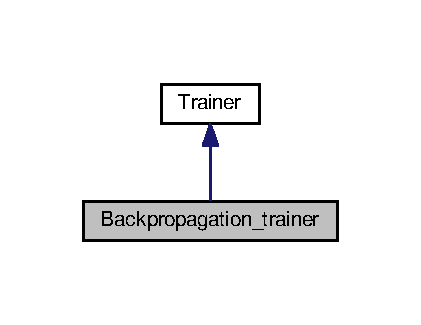
\includegraphics[width=202pt]{classBackpropagation__trainer__inherit__graph}
\end{center}
\end{figure}


Collaboration diagram for Backpropagation\-\_\-trainer\-:
\nopagebreak
\begin{figure}[H]
\begin{center}
\leavevmode
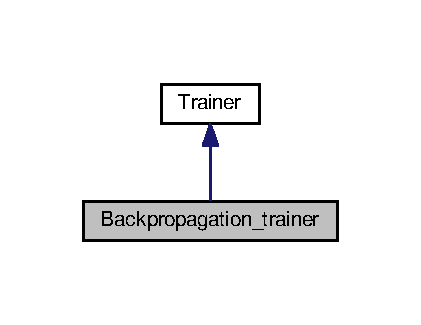
\includegraphics[width=202pt]{classBackpropagation__trainer__coll__graph}
\end{center}
\end{figure}
\subsection*{Public Member Functions}
\begin{DoxyCompactItemize}
\item 
\hypertarget{classBackpropagation__trainer_a06428f49ed527482daf4a0aa633a9ba7}{void {\bfseries train} (\hyperlink{classData__set}{Data\-\_\-set} data\-\_\-set, \hyperlink{classNeuralNet}{Neural\-Net} \&net)}\label{classBackpropagation__trainer_a06428f49ed527482daf4a0aa633a9ba7}

\item 
\hypertarget{classBackpropagation__trainer_a92736ecef749b201f345d9431b8ce810}{void {\bfseries train} (\hyperlink{classData__set}{Data\-\_\-set} data\-\_\-set, \hyperlink{classNeuralNet}{Neural\-Net} \&net, mat \&results\-\_\-cost\-\_\-and\-\_\-score\-\_\-evolution)}\label{classBackpropagation__trainer_a92736ecef749b201f345d9431b8ce810}

\end{DoxyCompactItemize}
\subsection*{Additional Inherited Members}


The documentation for this class was generated from the following files\-:\begin{DoxyCompactItemize}
\item 
backpropagation\-\_\-trainer.\-h\item 
backpropagation\-\_\-trainer.\-cpp\end{DoxyCompactItemize}

\hypertarget{classData__set}{\section{Data\-\_\-set Class Reference}
\label{classData__set}\index{Data\-\_\-set@{Data\-\_\-set}}
}


Collaboration diagram for Data\-\_\-set\-:
\nopagebreak
\begin{figure}[H]
\begin{center}
\leavevmode
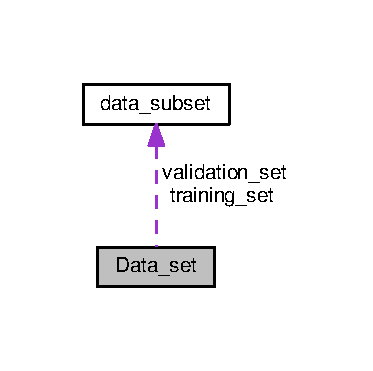
\includegraphics[width=179pt]{classData__set__coll__graph}
\end{center}
\end{figure}
\subsection*{Public Member Functions}
\begin{DoxyCompactItemize}
\item 
\hypertarget{classData__set_af0f3dbdff54b11ac32673376bae08496}{{\bfseries Data\-\_\-set} (unsigned int data\-\_\-set\-\_\-index)}\label{classData__set_af0f3dbdff54b11ac32673376bae08496}

\item 
\hypertarget{classData__set_a92c3a43a0975eb21124e7bcc97929e0a}{{\bfseries Data\-\_\-set} (string full\-\_\-path)}\label{classData__set_a92c3a43a0975eb21124e7bcc97929e0a}

\item 
\hypertarget{classData__set_aa7248d572372d35290301b9b99430e3e}{void {\bfseries select\-\_\-data\-\_\-set} (unsigned int chosen\-\_\-data\-\_\-set\-\_\-index, string \&data\-\_\-set\-\_\-filename, string \&octave\-\_\-variable\-\_\-name\-\_\-performances\-\_\-\-V\-S\-\_\-nb\-\_\-epochs, string \&octave\-\_\-variable\-\_\-name\-\_\-cost\-\_\-training\-\_\-set\-\_\-size, string \&octave\-\_\-variable\-\_\-name\-\_\-cost\-\_\-validation\-\_\-set\-\_\-size, string \&octave\-\_\-variable\-\_\-name\-\_\-scores\-\_\-pop\-\_\-size, string \&result\-\_\-filename)}\label{classData__set_aa7248d572372d35290301b9b99430e3e}

\item 
\hypertarget{classData__set_aa432606c593fd250c0a0ab609b66e444}{void {\bfseries set\-\_\-data\-\_\-set} (unsigned int chosen\-\_\-data\-\_\-set\-\_\-index, string \&data\-\_\-set\-\_\-filename)}\label{classData__set_aa432606c593fd250c0a0ab609b66e444}

\item 
\hypertarget{classData__set_ac7a6c8ad0589a66b22f60eb060bb78ea}{string {\bfseries get\-\_\-data\-\_\-set\-\_\-info} (mat data\-\_\-set)}\label{classData__set_ac7a6c8ad0589a66b22f60eb060bb78ea}

\item 
\hypertarget{classData__set_a349e7a0dde59198defde4ac0776417d6}{void {\bfseries subdivide\-\_\-data\-\_\-cross\-\_\-validation} (unsigned int index\-\_\-validation\-\_\-fold, unsigned int nb\-\_\-folds)}\label{classData__set_a349e7a0dde59198defde4ac0776417d6}

\end{DoxyCompactItemize}
\subsection*{Public Attributes}
\begin{DoxyCompactItemize}
\item 
\hypertarget{classData__set_a444ea0fda470430466122ccdbfc42c2b}{mat {\bfseries data}}\label{classData__set_a444ea0fda470430466122ccdbfc42c2b}

\item 
\hypertarget{classData__set_acb89adb39b0cdac43c7aa3f64223088d}{\hyperlink{structdata__subset}{data\-\_\-subset} {\bfseries training\-\_\-set}}\label{classData__set_acb89adb39b0cdac43c7aa3f64223088d}

\item 
\hypertarget{classData__set_a4ca480f137e45afbdefae9e6ec14aa9e}{\hyperlink{structdata__subset}{data\-\_\-subset} {\bfseries validation\-\_\-set}}\label{classData__set_a4ca480f137e45afbdefae9e6ec14aa9e}

\end{DoxyCompactItemize}


The documentation for this class was generated from the following files\-:\begin{DoxyCompactItemize}
\item 
data\-\_\-set.\-h\item 
data\-\_\-set.\-cpp\end{DoxyCompactItemize}

\hypertarget{structdata__subset}{\section{data\-\_\-subset Struct Reference}
\label{structdata__subset}\index{data\-\_\-subset@{data\-\_\-subset}}
}
\subsection*{Public Attributes}
\begin{DoxyCompactItemize}
\item 
\hypertarget{structdata__subset_a4e9c628ca7bc068e9f07e344afb5e2e1}{mat {\bfseries X}}\label{structdata__subset_a4e9c628ca7bc068e9f07e344afb5e2e1}

\item 
\hypertarget{structdata__subset_a5bfef53f9f76bd6a5252be74573c2a48}{mat {\bfseries Y}}\label{structdata__subset_a5bfef53f9f76bd6a5252be74573c2a48}

\end{DoxyCompactItemize}


The documentation for this struct was generated from the following file\-:\begin{DoxyCompactItemize}
\item 
data\-\_\-set.\-h\end{DoxyCompactItemize}

\hypertarget{classEvolutionary__trainer}{\section{Evolutionary\-\_\-trainer Class Reference}
\label{classEvolutionary__trainer}\index{Evolutionary\-\_\-trainer@{Evolutionary\-\_\-trainer}}
}


Inheritance diagram for Evolutionary\-\_\-trainer\-:
\nopagebreak
\begin{figure}[H]
\begin{center}
\leavevmode
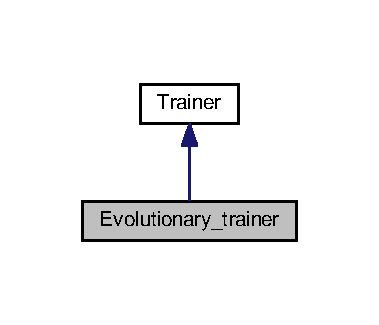
\includegraphics[width=182pt]{classEvolutionary__trainer__inherit__graph}
\end{center}
\end{figure}


Collaboration diagram for Evolutionary\-\_\-trainer\-:
\nopagebreak
\begin{figure}[H]
\begin{center}
\leavevmode
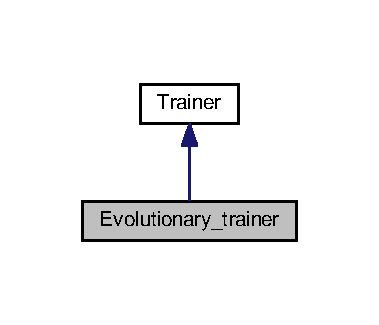
\includegraphics[width=182pt]{classEvolutionary__trainer__coll__graph}
\end{center}
\end{figure}
\subsection*{Public Member Functions}
\begin{DoxyCompactItemize}
\item 
\hypertarget{classEvolutionary__trainer_a79cc78bf8b6ecd051b5f49635e2fdf45}{void {\bfseries train} (\hyperlink{classData__set}{Data\-\_\-set} data\-\_\-set, \hyperlink{classNeuralNet}{Neural\-Net} \&net)}\label{classEvolutionary__trainer_a79cc78bf8b6ecd051b5f49635e2fdf45}

\item 
\hypertarget{classEvolutionary__trainer_a9c10b24b701858b8b03093deb31b9e47}{void {\bfseries train} (\hyperlink{classData__set}{Data\-\_\-set} data\-\_\-set, \hyperlink{classNeuralNet}{Neural\-Net} \&net, mat \&results\-\_\-score\-\_\-evolution)}\label{classEvolutionary__trainer_a9c10b24b701858b8b03093deb31b9e47}

\item 
\hypertarget{classEvolutionary__trainer_af39aecaac59934a47705c8b30de0b1ff}{void {\bfseries train\-\_\-weights} (\hyperlink{structdata__subset}{data\-\_\-subset} training\-\_\-set, \hyperlink{structdata__subset}{data\-\_\-subset} validation\-\_\-set, \hyperlink{classNeuralNet}{Neural\-Net} \&net, unsigned int nb\-\_\-epochs, mat \&results\-\_\-score\-\_\-evolution)}\label{classEvolutionary__trainer_af39aecaac59934a47705c8b30de0b1ff}

\item 
\hypertarget{classEvolutionary__trainer_a4793d8d79f60a25b20b7d7fc4be88294}{\hyperlink{classNeuralNet}{Neural\-Net} {\bfseries train\-\_\-topology\-\_\-plus\-\_\-weights} (\hyperlink{classData__set}{Data\-\_\-set} data\-\_\-set, \hyperlink{structnet__topology}{net\-\_\-topology} max\-\_\-topo, mat \&results\-\_\-score\-\_\-evolution)}\label{classEvolutionary__trainer_a4793d8d79f60a25b20b7d7fc4be88294}

\item 
\hypertarget{classEvolutionary__trainer_a208e5af359c6062733d96d17a95b46b8}{\hyperlink{classNeuralNet}{Neural\-Net} {\bfseries cross\-\_\-validation\-\_\-training} (\hyperlink{classData__set}{Data\-\_\-set} data\-\_\-set, \hyperlink{structnet__topology}{net\-\_\-topology} min\-\_\-topo, \hyperlink{structnet__topology}{net\-\_\-topology} max\-\_\-topo, mat \&results\-\_\-score\-\_\-evolution, double \&avrg\-\_\-score)}\label{classEvolutionary__trainer_a208e5af359c6062733d96d17a95b46b8}

\item 
\hyperlink{classNeuralNet}{Neural\-Net} \hyperlink{classEvolutionary__trainer_aee8c215b6f8cea925138f736f35413e8}{evolve\-\_\-through\-\_\-generations} (\hyperlink{structdata__subset}{data\-\_\-subset} training\-\_\-set, \hyperlink{structnet__topology}{net\-\_\-topology} min\-\_\-topo, \hyperlink{structnet__topology}{net\-\_\-topology} max\-\_\-topo, unsigned int nb\-\_\-epochs, mat \&results\-\_\-cost\-\_\-and\-\_\-score\-\_\-evolution, unsigned int index\-\_\-cross\-\_\-validation\-\_\-section)
\item 
\hypertarget{classEvolutionary__trainer_a46fd9af5bb456a2cbc4621f5a0f6d3e5}{void {\bfseries generate\-\_\-random\-\_\-population} (unsigned int pop\-\_\-size, \hyperlink{structnet__topology}{net\-\_\-topology} max\-\_\-topo)}\label{classEvolutionary__trainer_a46fd9af5bb456a2cbc4621f5a0f6d3e5}

\item 
\hypertarget{classEvolutionary__trainer_af99a07cfacf9ba82026ea175eb9a58e8}{\hyperlink{classNeuralNet}{Neural\-Net} {\bfseries get\-\_\-best\-\_\-model} (vector$<$ \hyperlink{classNeuralNet}{Neural\-Net} $>$ pop)}\label{classEvolutionary__trainer_af99a07cfacf9ba82026ea175eb9a58e8}

\item 
\hypertarget{classEvolutionary__trainer_a592e3ac8186cb753aa6657d10071b21b}{\hyperlink{classNeuralNet}{Neural\-Net} {\bfseries get\-\_\-best\-\_\-model} (vector$<$ vec $>$ genome\-\_\-pop)}\label{classEvolutionary__trainer_a592e3ac8186cb753aa6657d10071b21b}

\item 
\hypertarget{classEvolutionary__trainer_a0165542480e5b3209d7566ced1079960}{vec {\bfseries get\-\_\-genome} (\hyperlink{classNeuralNet}{Neural\-Net} n, \hyperlink{structnet__topology}{net\-\_\-topology} largest\-\_\-topology)}\label{classEvolutionary__trainer_a0165542480e5b3209d7566ced1079960}

\item 
\hypertarget{classEvolutionary__trainer_a0d49a904e77b9bb62c43bdf643b1d508}{\hyperlink{classNeuralNet}{Neural\-Net} {\bfseries generate\-\_\-net} (vec genome)}\label{classEvolutionary__trainer_a0d49a904e77b9bb62c43bdf643b1d508}

\item 
\hypertarget{classEvolutionary__trainer_a7c4e15cd59c8f37c0483625a94a2fb75}{unsigned int {\bfseries get\-\_\-genome\-\_\-length} (\hyperlink{structnet__topology}{net\-\_\-topology} t)}\label{classEvolutionary__trainer_a7c4e15cd59c8f37c0483625a94a2fb75}

\item 
\hypertarget{classEvolutionary__trainer_ace69491101081a9efad446900975a32c}{unsigned int {\bfseries get\-\_\-population\-\_\-size} ()}\label{classEvolutionary__trainer_ace69491101081a9efad446900975a32c}

\item 
\hypertarget{classEvolutionary__trainer_ae6e1cc7504247c515efb79f483d11cb5}{mat {\bfseries get\-\_\-population\-\_\-scores} (\hyperlink{structdata__subset}{data\-\_\-subset} d)}\label{classEvolutionary__trainer_ae6e1cc7504247c515efb79f483d11cb5}

\item 
\hypertarget{classEvolutionary__trainer_a87eacfa4ce8c6482b4c7b86529e00caa}{vector$<$ \hyperlink{classNeuralNet}{Neural\-Net} $>$ {\bfseries get\-\_\-population} ()}\label{classEvolutionary__trainer_a87eacfa4ce8c6482b4c7b86529e00caa}

\item 
\hypertarget{classEvolutionary__trainer_ad0778d747295796e9c4f82a1bb20ca70}{void {\bfseries set\-\_\-population} (vector$<$ \hyperlink{classNeuralNet}{Neural\-Net} $>$ pop)}\label{classEvolutionary__trainer_ad0778d747295796e9c4f82a1bb20ca70}

\item 
\hypertarget{classEvolutionary__trainer_abd389f2edff316fe4acd0a29b10156ec}{void {\bfseries insert\-\_\-individual} (\hyperlink{classNeuralNet}{Neural\-Net} indiv)}\label{classEvolutionary__trainer_abd389f2edff316fe4acd0a29b10156ec}

\end{DoxyCompactItemize}
\subsection*{Additional Inherited Members}


\subsection{Member Function Documentation}
\hypertarget{classEvolutionary__trainer_aee8c215b6f8cea925138f736f35413e8}{\index{Evolutionary\-\_\-trainer@{Evolutionary\-\_\-trainer}!evolve\-\_\-through\-\_\-generations@{evolve\-\_\-through\-\_\-generations}}
\index{evolve\-\_\-through\-\_\-generations@{evolve\-\_\-through\-\_\-generations}!Evolutionary_trainer@{Evolutionary\-\_\-trainer}}
\subsubsection[{evolve\-\_\-through\-\_\-generations}]{\setlength{\rightskip}{0pt plus 5cm}{\bf Neural\-Net} Evolutionary\-\_\-trainer\-::evolve\-\_\-through\-\_\-generations (
\begin{DoxyParamCaption}
\item[{{\bf data\-\_\-subset}}]{training\-\_\-set, }
\item[{{\bf net\-\_\-topology}}]{min\-\_\-topo, }
\item[{{\bf net\-\_\-topology}}]{max\-\_\-topo, }
\item[{unsigned int}]{nb\-\_\-epochs, }
\item[{mat \&}]{results\-\_\-cost\-\_\-and\-\_\-score\-\_\-evolution, }
\item[{unsigned int}]{index\-\_\-cross\-\_\-validation\-\_\-section}
\end{DoxyParamCaption}
)}}\label{classEvolutionary__trainer_aee8c215b6f8cea925138f736f35413e8}
R\-U\-N\-N\-I\-N\-G\-: Differential Evolution

T\-E\-R\-M\-I\-N\-A\-T\-I\-O\-N C\-R\-I\-T\-E\-R\-I\-O\-N\-: If all generations were achieved O\-R if the G\-A has already converged

The documentation for this class was generated from the following files\-:\begin{DoxyCompactItemize}
\item 
evolutionary\-\_\-trainer.\-h\item 
evolutionary\-\_\-trainer.\-cpp\end{DoxyCompactItemize}

\hypertarget{classinvalid__dataset__exception}{\section{invalid\-\_\-dataset\-\_\-exception Class Reference}
\label{classinvalid__dataset__exception}\index{invalid\-\_\-dataset\-\_\-exception@{invalid\-\_\-dataset\-\_\-exception}}
}


Inheritance diagram for invalid\-\_\-dataset\-\_\-exception\-:
\nopagebreak
\begin{figure}[H]
\begin{center}
\leavevmode
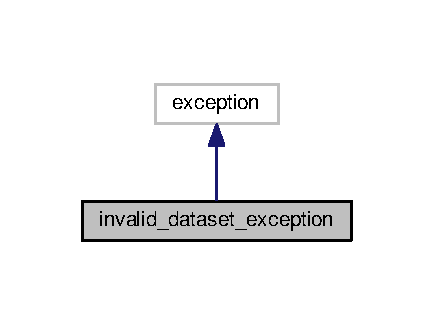
\includegraphics[width=208pt]{classinvalid__dataset__exception__inherit__graph}
\end{center}
\end{figure}


Collaboration diagram for invalid\-\_\-dataset\-\_\-exception\-:
\nopagebreak
\begin{figure}[H]
\begin{center}
\leavevmode
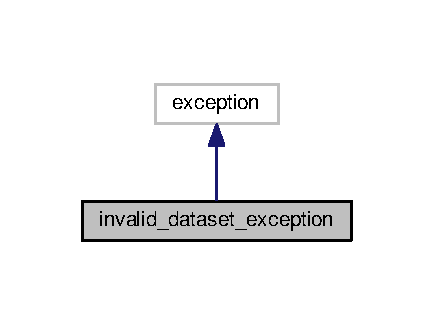
\includegraphics[width=208pt]{classinvalid__dataset__exception__coll__graph}
\end{center}
\end{figure}


The documentation for this class was generated from the following file\-:\begin{DoxyCompactItemize}
\item 
data\-\_\-set.\-h\end{DoxyCompactItemize}

\hypertarget{classNet__benchmark}{\section{Net\-\_\-benchmark Class Reference}
\label{classNet__benchmark}\index{Net\-\_\-benchmark@{Net\-\_\-benchmark}}
}
\subsection*{Public Member Functions}
\begin{DoxyCompactItemize}
\item 
\hypertarget{classNet__benchmark_ad82d3a4ec7f72525398b912e6f2adb6f}{void {\bfseries run\-\_\-benchmark} (unsigned int nb\-\_\-rep)}\label{classNet__benchmark_ad82d3a4ec7f72525398b912e6f2adb6f}

\item 
\hypertarget{classNet__benchmark_aa1416831a6e196d4297fcc8d3261c790}{void {\bfseries train\-\_\-topology} (\hyperlink{classNeuralNet}{Neural\-Net} \&net)}\label{classNet__benchmark_aa1416831a6e196d4297fcc8d3261c790}

\item 
\hypertarget{classNet__benchmark_a5ad4944768cd84b18c97e33950fa6ee7}{void {\bfseries set\-\_\-topology} (\hyperlink{structnet__topology}{net\-\_\-topology} t)}\label{classNet__benchmark_a5ad4944768cd84b18c97e33950fa6ee7}

\item 
\hypertarget{classNet__benchmark_a39cebf7409dc8665b3a11a2c3bf79076}{void {\bfseries compute\-\_\-perfs\-\_\-test\-\_\-validation} (double \&model\-\_\-score\-\_\-training\-\_\-set, double \&model\-\_\-prediction\-\_\-accuracy\-\_\-training\-\_\-set, double \&model\-\_\-score\-\_\-validation\-\_\-set, double \&model\-\_\-prediction\-\_\-accuracy\-\_\-validation\-\_\-set)}\label{classNet__benchmark_a39cebf7409dc8665b3a11a2c3bf79076}

\end{DoxyCompactItemize}


The documentation for this class was generated from the following files\-:\begin{DoxyCompactItemize}
\item 
net\-\_\-benchmark.\-h\item 
net\-\_\-benchmark.\-cpp\end{DoxyCompactItemize}

\hypertarget{structnet__topology}{\section{net\-\_\-topology Struct Reference}
\label{structnet__topology}\index{net\-\_\-topology@{net\-\_\-topology}}
}
\subsection*{Public Member Functions}
\begin{DoxyCompactItemize}
\item 
\hypertarget{structnet__topology_af25fe4ae6c2f5d74a975c0706d9f8961}{unsigned int {\bfseries get\-\_\-total\-\_\-nb\-\_\-weights} ()}\label{structnet__topology_af25fe4ae6c2f5d74a975c0706d9f8961}

\item 
\hypertarget{structnet__topology_a4160d0c5538ffdd2d3dca43be63f4dd2}{string {\bfseries to\-\_\-string} ()}\label{structnet__topology_a4160d0c5538ffdd2d3dca43be63f4dd2}

\end{DoxyCompactItemize}
\subsection*{Public Attributes}
\begin{DoxyCompactItemize}
\item 
\hypertarget{structnet__topology_a345bfe167c9ad673ce83f524d16e2e60}{unsigned int {\bfseries nb\-\_\-input\-\_\-units}}\label{structnet__topology_a345bfe167c9ad673ce83f524d16e2e60}

\item 
\hypertarget{structnet__topology_a469559ffc92c5db31d01ab57814662a8}{unsigned int {\bfseries nb\-\_\-units\-\_\-per\-\_\-hidden\-\_\-layer}}\label{structnet__topology_a469559ffc92c5db31d01ab57814662a8}

\item 
\hypertarget{structnet__topology_a56a9faef666829e261bb23fc6b0ccc53}{unsigned int {\bfseries nb\-\_\-output\-\_\-units}}\label{structnet__topology_a56a9faef666829e261bb23fc6b0ccc53}

\item 
\hypertarget{structnet__topology_a3efe7d1cda6f053c1377d4c2b403dd2c}{unsigned int {\bfseries nb\-\_\-hidden\-\_\-layers}}\label{structnet__topology_a3efe7d1cda6f053c1377d4c2b403dd2c}

\end{DoxyCompactItemize}


The documentation for this struct was generated from the following file\-:\begin{DoxyCompactItemize}
\item 
neuralnet.\-h\end{DoxyCompactItemize}

\hypertarget{classNeuralNet}{\section{Neural\-Net Class Reference}
\label{classNeuralNet}\index{Neural\-Net@{Neural\-Net}}
}


The \hyperlink{classNeuralNet}{Neural\-Net} class.  




{\ttfamily \#include $<$neuralnet.\-h$>$}

\subsection*{Public Member Functions}
\begin{DoxyCompactItemize}
\item 
\hypertarget{classNeuralNet_aea0e1ca0f36640971b2954d135b0a12e}{{\bfseries Neural\-Net} (\hyperlink{structnet__topology}{net\-\_\-topology} t)}\label{classNeuralNet_aea0e1ca0f36640971b2954d135b0a12e}

\item 
mat \hyperlink{classNeuralNet_ab53c509b46f5a901a45be9e4cf77f3bd}{forward\-\_\-propagate} (mat X)
\begin{DoxyCompactList}\small\item\em forward\-\_\-propagate \end{DoxyCompactList}\item 
mat \hyperlink{classNeuralNet_a6a9fdc8fffbd2745d7cca5562912335b}{forward\-\_\-propagate} (mat X, vector$<$ mat $>$ \&Zs, vector$<$ mat $>$ \&As)
\begin{DoxyCompactList}\small\item\em forward\-\_\-propagate \end{DoxyCompactList}\item 
vector$<$ mat $>$ \hyperlink{classNeuralNet_a74dc26bcfbb7a054a8c7697f537a5a99}{reshape\-\_\-weights} ()
\begin{DoxyCompactList}\small\item\em reshape\-\_\-weights \end{DoxyCompactList}\item 
\hypertarget{classNeuralNet_aefd889aaa736267ae67bd2beb0275628}{void {\bfseries save\-\_\-net} (ofstream \&model\-\_\-file)}\label{classNeuralNet_aefd889aaa736267ae67bd2beb0275628}

\item 
\hypertarget{classNeuralNet_a2e458054a038980589c2c4a97e647709}{unsigned int {\bfseries get\-\_\-total\-\_\-nb\-\_\-weights} ()}\label{classNeuralNet_a2e458054a038980589c2c4a97e647709}

\item 
\hypertarget{classNeuralNet_ae24cbf6ab4032ca16983dbed084b6d85}{vec {\bfseries generate\-\_\-random\-\_\-model} ()}\label{classNeuralNet_ae24cbf6ab4032ca16983dbed084b6d85}

\item 
\hypertarget{classNeuralNet_a7749da58906658bed5b008c6022807ee}{void {\bfseries print\-\_\-topology} ()}\label{classNeuralNet_a7749da58906658bed5b008c6022807ee}

\item 
\hypertarget{classNeuralNet_a41636bc3b34948ad3da08980af76387d}{vec {\bfseries get\-\_\-params} ()}\label{classNeuralNet_a41636bc3b34948ad3da08980af76387d}

\item 
\hypertarget{classNeuralNet_af9a25d684ca80c51953bfef7fd443e2d}{void {\bfseries set\-\_\-params} (vec p)}\label{classNeuralNet_af9a25d684ca80c51953bfef7fd443e2d}

\item 
\hypertarget{classNeuralNet_ad32dd2df156318945f665949f1759875}{\hyperlink{structnet__topology}{net\-\_\-topology} {\bfseries get\-\_\-topology} ()}\label{classNeuralNet_ad32dd2df156318945f665949f1759875}

\item 
\hypertarget{classNeuralNet_a241e0975c735bff8804fe42a205d0b39}{void {\bfseries set\-\_\-topology} (\hyperlink{structnet__topology}{net\-\_\-topology} t)}\label{classNeuralNet_a241e0975c735bff8804fe42a205d0b39}

\item 
double \hyperlink{classNeuralNet_ab7227a1d2bebbc92c1c7dc5a952ad2cc}{get\-\_\-accuracy} (\hyperlink{structdata__subset}{data\-\_\-subset} d)
\begin{DoxyCompactList}\small\item\em get\-\_\-accuracy \end{DoxyCompactList}\item 
double \hyperlink{classNeuralNet_aecea67ed4059c88b0b74c13f0c7c52a7}{get\-\_\-f1\-\_\-score} (\hyperlink{structdata__subset}{data\-\_\-subset} d)
\begin{DoxyCompactList}\small\item\em get\-\_\-f1\-\_\-score \end{DoxyCompactList}\item 
double \hyperlink{classNeuralNet_a97703e2851b62dbdd0ded415542d8614}{get\-\_\-matthews\-\_\-correlation\-\_\-coefficient} (\hyperlink{structdata__subset}{data\-\_\-subset} d)
\begin{DoxyCompactList}\small\item\em get\-\_\-matthews\-\_\-correlation\-\_\-coefficient \end{DoxyCompactList}\item 
\hypertarget{classNeuralNet_adc22e85172dc8cd50ebcda46d8b9ba58}{void {\bfseries print\-\_\-topology} (\hyperlink{structnet__topology}{net\-\_\-topology} t)}\label{classNeuralNet_adc22e85172dc8cd50ebcda46d8b9ba58}

\item 
bool \hyperlink{classNeuralNet_a3f74539900212d97ed0eeb8117613943}{operator$<$} (\hyperlink{classNeuralNet}{Neural\-Net} \&n)
\begin{DoxyCompactList}\small\item\em operator $<$ (comparator-\/function for sorting by highest score) \end{DoxyCompactList}\end{DoxyCompactItemize}


\subsection{Detailed Description}
The \hyperlink{classNeuralNet}{Neural\-Net} class. 

\subsection{Member Function Documentation}
\hypertarget{classNeuralNet_ab53c509b46f5a901a45be9e4cf77f3bd}{\index{Neural\-Net@{Neural\-Net}!forward\-\_\-propagate@{forward\-\_\-propagate}}
\index{forward\-\_\-propagate@{forward\-\_\-propagate}!NeuralNet@{Neural\-Net}}
\subsubsection[{forward\-\_\-propagate}]{\setlength{\rightskip}{0pt plus 5cm}mat Neural\-Net\-::forward\-\_\-propagate (
\begin{DoxyParamCaption}
\item[{mat}]{X}
\end{DoxyParamCaption}
)}}\label{classNeuralNet_ab53c509b46f5a901a45be9e4cf77f3bd}


forward\-\_\-propagate 


\begin{DoxyParams}{Parameters}
{\em X} & Input data as matrix, whether it contains a single row or several. (Must fit the number of input neurons) \\
\hline
\end{DoxyParams}
\begin{DoxyReturn}{Returns}
The predictions made by the net on the input data X 
\end{DoxyReturn}
\hypertarget{classNeuralNet_a6a9fdc8fffbd2745d7cca5562912335b}{\index{Neural\-Net@{Neural\-Net}!forward\-\_\-propagate@{forward\-\_\-propagate}}
\index{forward\-\_\-propagate@{forward\-\_\-propagate}!NeuralNet@{Neural\-Net}}
\subsubsection[{forward\-\_\-propagate}]{\setlength{\rightskip}{0pt plus 5cm}mat Neural\-Net\-::forward\-\_\-propagate (
\begin{DoxyParamCaption}
\item[{mat}]{X, }
\item[{vector$<$ mat $>$ \&}]{Zs, }
\item[{vector$<$ mat $>$ \&}]{As}
\end{DoxyParamCaption}
)}}\label{classNeuralNet_a6a9fdc8fffbd2745d7cca5562912335b}


forward\-\_\-propagate 


\begin{DoxyParams}{Parameters}
{\em X} & Input data as matrix, whether it contains a single row or several. (Must fit the number of input neurons) \\
\hline
{\em Zs} & vector of matrices for the summed weights$\ast$inputs(not yet been through sigmoid) to be returned by reference \\
\hline
{\em As} & vector of matrices for the activations (outputs) of the neurons to be returned by reference \\
\hline
\end{DoxyParams}
\begin{DoxyReturn}{Returns}
The predictions made by the net on the input data X Also returns (by reference) the updated state of the vectors Z and A 
\end{DoxyReturn}
\hypertarget{classNeuralNet_ab7227a1d2bebbc92c1c7dc5a952ad2cc}{\index{Neural\-Net@{Neural\-Net}!get\-\_\-accuracy@{get\-\_\-accuracy}}
\index{get\-\_\-accuracy@{get\-\_\-accuracy}!NeuralNet@{Neural\-Net}}
\subsubsection[{get\-\_\-accuracy}]{\setlength{\rightskip}{0pt plus 5cm}double Neural\-Net\-::get\-\_\-accuracy (
\begin{DoxyParamCaption}
\item[{{\bf data\-\_\-subset}}]{d}
\end{DoxyParamCaption}
)}}\label{classNeuralNet_ab7227a1d2bebbc92c1c7dc5a952ad2cc}


get\-\_\-accuracy 


\begin{DoxyParams}{Parameters}
{\em d} & data portion used for accuracy calculation \\
\hline
\end{DoxyParams}
\begin{DoxyReturn}{Returns}
returns percentage representing how often the model correctly predicts $<$\-Y$>$ on the data-\/set $<$\-X$>$ 
\end{DoxyReturn}
\hypertarget{classNeuralNet_aecea67ed4059c88b0b74c13f0c7c52a7}{\index{Neural\-Net@{Neural\-Net}!get\-\_\-f1\-\_\-score@{get\-\_\-f1\-\_\-score}}
\index{get\-\_\-f1\-\_\-score@{get\-\_\-f1\-\_\-score}!NeuralNet@{Neural\-Net}}
\subsubsection[{get\-\_\-f1\-\_\-score}]{\setlength{\rightskip}{0pt plus 5cm}double Neural\-Net\-::get\-\_\-f1\-\_\-score (
\begin{DoxyParamCaption}
\item[{{\bf data\-\_\-subset}}]{d}
\end{DoxyParamCaption}
)}}\label{classNeuralNet_aecea67ed4059c88b0b74c13f0c7c52a7}


get\-\_\-f1\-\_\-score 


\begin{DoxyParams}{Parameters}
{\em d} & \\
\hline
\end{DoxyParams}
\begin{DoxyReturn}{Returns}
(score function) returns an indication of the quality of the model \mbox{[}0, 1\mbox{]} The F1 Score function calculates the {\itshape precision} and {\itshape recall} of the model. This function is used as fitness function by the Differential Evolution algorithm. 
\end{DoxyReturn}
\hypertarget{classNeuralNet_a97703e2851b62dbdd0ded415542d8614}{\index{Neural\-Net@{Neural\-Net}!get\-\_\-matthews\-\_\-correlation\-\_\-coefficient@{get\-\_\-matthews\-\_\-correlation\-\_\-coefficient}}
\index{get\-\_\-matthews\-\_\-correlation\-\_\-coefficient@{get\-\_\-matthews\-\_\-correlation\-\_\-coefficient}!NeuralNet@{Neural\-Net}}
\subsubsection[{get\-\_\-matthews\-\_\-correlation\-\_\-coefficient}]{\setlength{\rightskip}{0pt plus 5cm}double Neural\-Net\-::get\-\_\-matthews\-\_\-correlation\-\_\-coefficient (
\begin{DoxyParamCaption}
\item[{{\bf data\-\_\-subset}}]{d}
\end{DoxyParamCaption}
)}}\label{classNeuralNet_a97703e2851b62dbdd0ded415542d8614}


get\-\_\-matthews\-\_\-correlation\-\_\-coefficient 


\begin{DoxyParams}{Parameters}
{\em d} & \\
\hline
\end{DoxyParams}
\begin{DoxyReturn}{Returns}
(score function) returns an indication of the quality of the model \mbox{[}-\/1, +1\mbox{]} 
\end{DoxyReturn}
\hypertarget{classNeuralNet_a3f74539900212d97ed0eeb8117613943}{\index{Neural\-Net@{Neural\-Net}!operator$<$@{operator$<$}}
\index{operator$<$@{operator$<$}!NeuralNet@{Neural\-Net}}
\subsubsection[{operator$<$}]{\setlength{\rightskip}{0pt plus 5cm}bool Neural\-Net\-::operator$<$ (
\begin{DoxyParamCaption}
\item[{{\bf Neural\-Net} \&}]{n}
\end{DoxyParamCaption}
)\hspace{0.3cm}{\ttfamily [inline]}}}\label{classNeuralNet_a3f74539900212d97ed0eeb8117613943}


operator $<$ (comparator-\/function for sorting by highest score) 


\begin{DoxyParams}{Parameters}
{\em n} & \\
\hline
\end{DoxyParams}
\begin{DoxyReturn}{Returns}
true if the provided net is less fit than this net 
\end{DoxyReturn}
\hypertarget{classNeuralNet_a74dc26bcfbb7a054a8c7697f537a5a99}{\index{Neural\-Net@{Neural\-Net}!reshape\-\_\-weights@{reshape\-\_\-weights}}
\index{reshape\-\_\-weights@{reshape\-\_\-weights}!NeuralNet@{Neural\-Net}}
\subsubsection[{reshape\-\_\-weights}]{\setlength{\rightskip}{0pt plus 5cm}vector$<$ mat $>$ Neural\-Net\-::reshape\-\_\-weights (
\begin{DoxyParamCaption}
{}
\end{DoxyParamCaption}
)}}\label{classNeuralNet_a74dc26bcfbb7a054a8c7697f537a5a99}


reshape\-\_\-weights 

\begin{DoxyReturn}{Returns}
returns vector of Theta (weights) matrices of the neural network e.\-g. if net has 1 input layer, 1 hidden layer, 1 output layer \hyperlink{classNeuralNet_a74dc26bcfbb7a054a8c7697f537a5a99}{reshape\-\_\-weights()} will return a vector of the two weight matrices respectively Theta\mbox{[}0\mbox{]} and Theta\mbox{[}1\mbox{]} 
\end{DoxyReturn}


The documentation for this class was generated from the following files\-:\begin{DoxyCompactItemize}
\item 
neuralnet.\-h\item 
neuralnet.\-cpp\end{DoxyCompactItemize}

\hypertarget{classTrainer}{\section{Trainer Class Reference}
\label{classTrainer}\index{Trainer@{Trainer}}
}


Inheritance diagram for Trainer\-:
\nopagebreak
\begin{figure}[H]
\begin{center}
\leavevmode
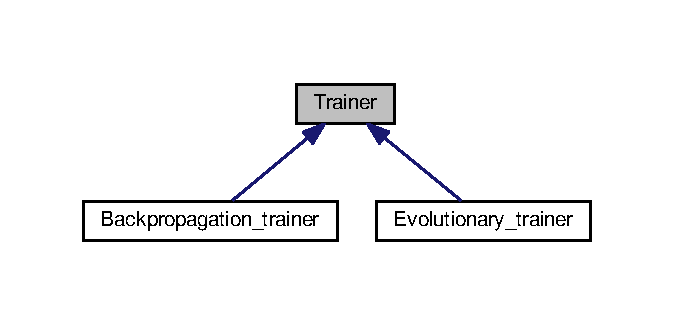
\includegraphics[width=323pt]{classTrainer__inherit__graph}
\end{center}
\end{figure}
\subsection*{Public Member Functions}
\begin{DoxyCompactItemize}
\item 
\hypertarget{classTrainer_a6e5d64b4e5647dc17d985fddfa96601d}{virtual void {\bfseries train} (\hyperlink{classData__set}{Data\-\_\-set} data\-\_\-set, \hyperlink{classNeuralNet}{Neural\-Net} \&net)=0}\label{classTrainer_a6e5d64b4e5647dc17d985fddfa96601d}

\item 
\hypertarget{classTrainer_a0ca142f63b8891a7fbd43054fbb59606}{virtual void {\bfseries train} (\hyperlink{classData__set}{Data\-\_\-set} data\-\_\-set, \hyperlink{classNeuralNet}{Neural\-Net} \&net, mat \&results\-\_\-cost\-\_\-and\-\_\-score\-\_\-evolution)=0}\label{classTrainer_a0ca142f63b8891a7fbd43054fbb59606}

\item 
\hypertarget{classTrainer_aa8218ae66628883d2125a8d627dbd2e7}{unsigned int {\bfseries get\-\_\-nb\-\_\-epochs} ()}\label{classTrainer_aa8218ae66628883d2125a8d627dbd2e7}

\item 
\hypertarget{classTrainer_a7c7c9b96a6f0cc94ee32f902abe4ec01}{void {\bfseries set\-\_\-nb\-\_\-epochs} (unsigned int e)}\label{classTrainer_a7c7c9b96a6f0cc94ee32f902abe4ec01}

\end{DoxyCompactItemize}
\subsection*{Protected Member Functions}
\begin{DoxyCompactItemize}
\item 
\hypertarget{classTrainer_ae39aafe6ffcb181ec7401e94d36c81b1}{unsigned int {\bfseries generate\-\_\-random\-\_\-integer\-\_\-between\-\_\-range} (unsigned int min, unsigned int max)}\label{classTrainer_ae39aafe6ffcb181ec7401e94d36c81b1}

\end{DoxyCompactItemize}
\subsection*{Protected Attributes}
\begin{DoxyCompactItemize}
\item 
\hypertarget{classTrainer_a7475106292815bd6c082945c6b090c6b}{unsigned int {\bfseries nb\-\_\-epochs}}\label{classTrainer_a7475106292815bd6c082945c6b090c6b}

\end{DoxyCompactItemize}


The documentation for this class was generated from the following files\-:\begin{DoxyCompactItemize}
\item 
trainer.\-h\item 
trainer.\-cpp\end{DoxyCompactItemize}

%--- End generated contents ---

% Index
\newpage
\phantomsection
\addcontentsline{toc}{chapter}{Index}
\printindex

\end{document}
